\documentclass[10pt]{beamer}
\usetheme[progressbar=frametitle]{metropolis}
\setbeamercovered{transparent}
\usepackage{appendixnumberbeamer}
\usepackage{booktabs}
\usepackage[scale=2]{ccicons}
\usepackage{pgfplots}
\usepackage{amssymb}
\usepackage{xspace}
\usepackage{mathtools}
\usepackage{graphicx}
\usepackage{subcaption}
\usepgfplotslibrary{dateplot}
\newcommand{\themename}{\textbf{\textsc{metropolis}}\xspace}
\usepackage[
backend=biber,
style=bwl-FU,
citestyle=bwl-FU
]{biblatex}
\addbibresource{bibliography.bib}
\geometry{paperwidth=180mm,paperheight=105mm}
\title{Regression Trees}
\author{Timothy Currie}
\institute{Universität Bonn}
\date{\vspace{2cm} \textbf{\large{Wissenschaftliches Arbeiten}} \\ \textbf{25/06/2024} \\ 
       \vspace{1cm} \textbf{Supervisor:} Dr. Elias Wolf \\ 
       \textbf{Matrikelnummer:} 50074426}
\begin{document}
\maketitle












\begin{frame}{Motivation}
    \begin{itemize}
        \item Linear regression performs poorly on many kinds of data.
        \item E.g. data with non-linear relationships and interaction effects.
        \item What might be a better approach for these situations?
            
        \item Regression Trees can be useful in many situations.
    \end{itemize}
 \begin{figure}
            \centering
            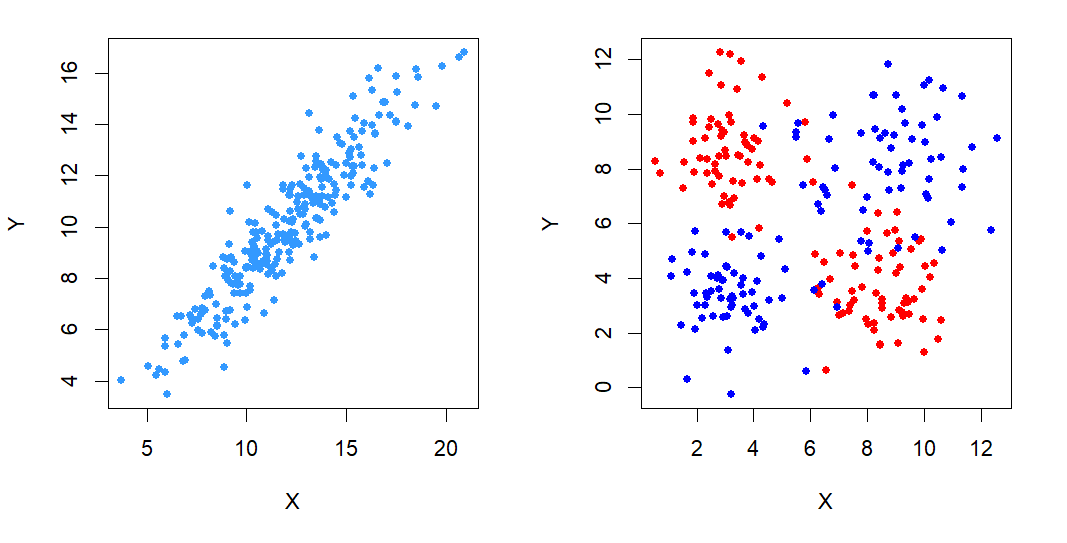
\includegraphics[scale=0.5]{Motivation Together.png}
            \caption{Can you guess where regression trees and where linear regression will perform better?}
            \label{fig:sub1}
        \end{figure}
\end{frame}






\begin{frame}{Outline of the Talk}
    \begin{large}
    \begin{enumerate}
        \item Motivation
        \item Basics of Regression Trees
        \item Comparing regression Trees and Linear Regression
        \item Overfitting and Pruning
        \item Ensemble methods and BART
        \item Conclusion
        \item References
    \end{enumerate}
    \end{large}
\end{frame}


\begin{frame}{Basics of Regression Trees}
    \begin{itemize}
        \item Regression trees split the predictor space into regions that minimize the RSS given by
    
    \begin{align*}
        \sum_{j=1}^{J} \sum_{i \in R_j} ( y_i- \hat{ y}_{R_j} )^2
    \end{align*}
    
    
    \item In each region $\hat{y}$ simply takes on the mean of all observations in that region.
    
        \item Typically we can't find the optimal regions.
        \item Instead we use a greedy algorithm \textbf{Recursive binary splitting} to find the optimal split to minimize prediction error at each stage.
        
        \vspace{1cm}
        \item \textbf{Main differences between linear regression and trees}
        \begin{itemize}
            \item Regression trees do not assume a linear relationship between predictors and the response.
        
            \item Trees capture interaction effects naturally.
        \end{itemize}
       
    \end{itemize}
\end{frame}


\begin{frame}{Simulation: Linear Data}
    \begin{columns}[T]
        \begin{column}{0.5\textwidth}
            \begin{figure}
            \centering
                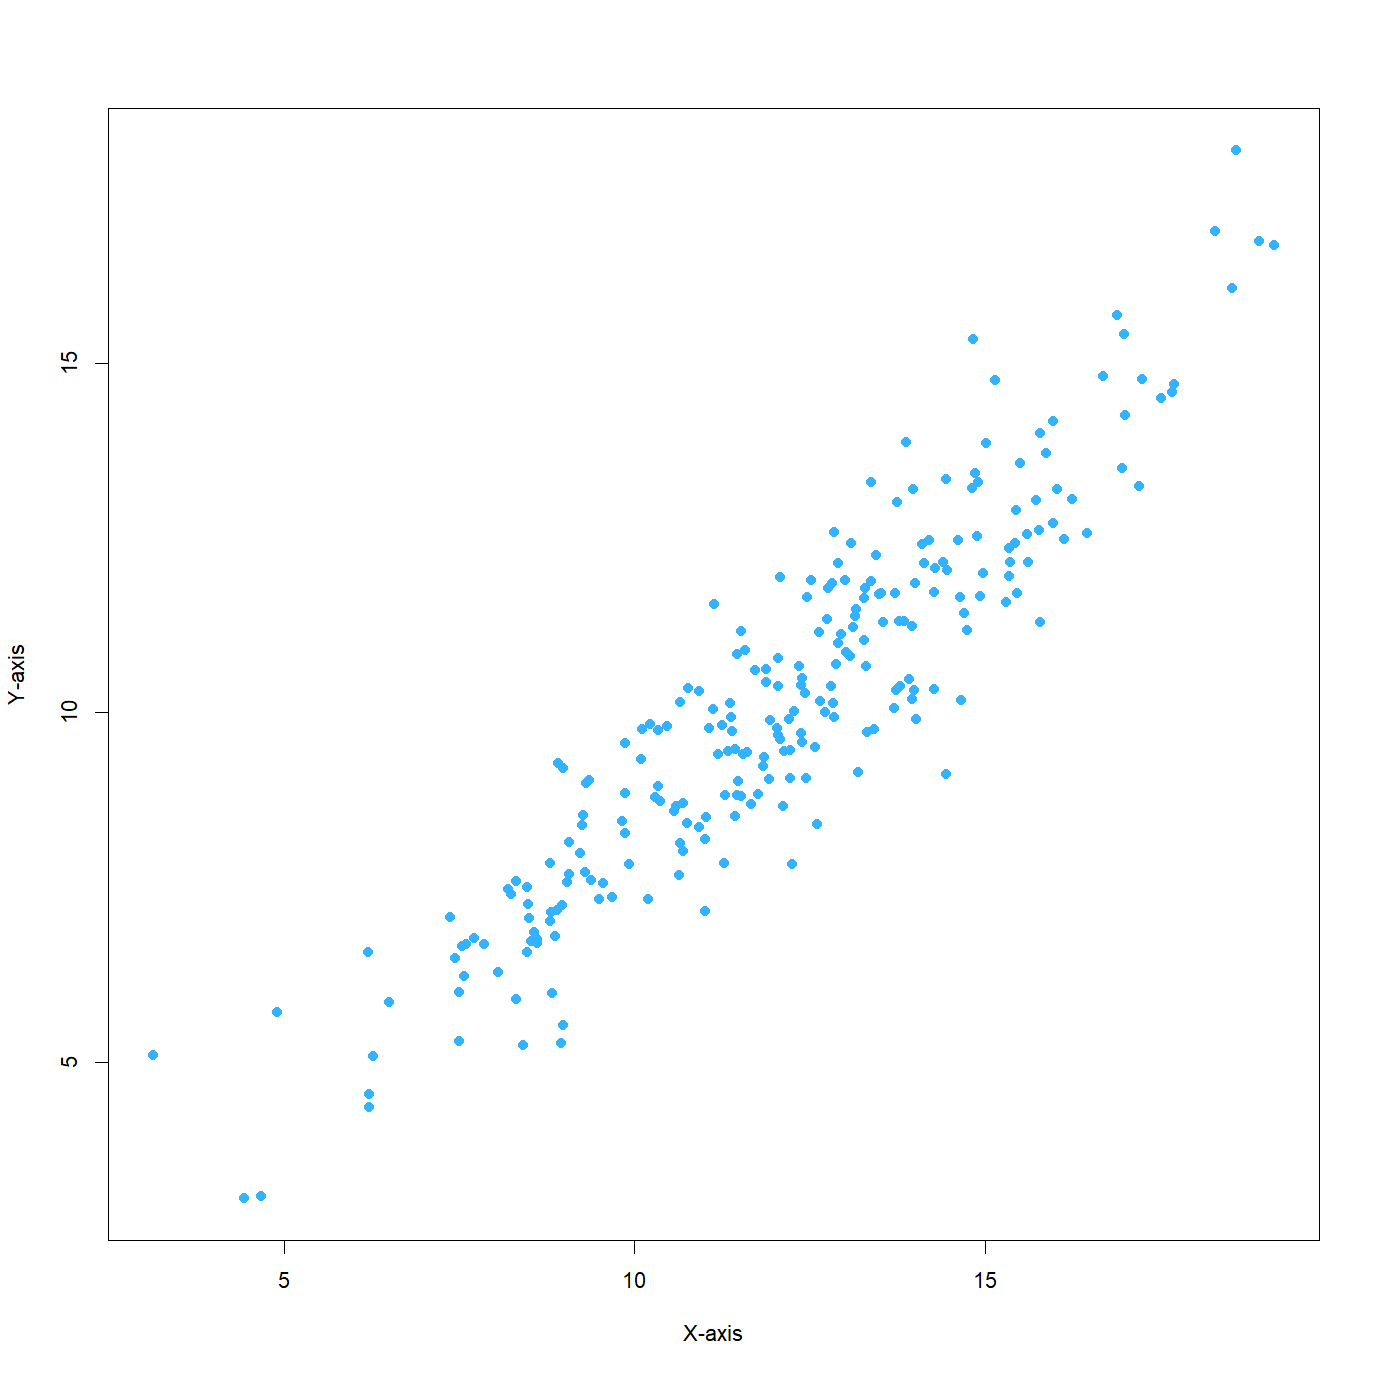
\includegraphics[width=1\linewidth]{Linear Data before.png}
                \caption{Linear Relation between Variables}
                \label{fig:sub2}  % Changed label to be unique
            \end{figure}
        \end{column}
        \begin{column}{0.5\textwidth}
            \begin{itemize}
            \vspace{0.7cm}
                \item We will run all simulations 400 times.
                 \item For now the regression trees will have 4 terminal Nodes.
                \item And we will always compare the Mean Squared Error (MSE).
                \item Data generated as: $Y = \beta_0 + \beta_1X + \epsilon$
                \item Where $\epsilon \sim N(0, \sigma^2)$
            \end{itemize}
        \end{column}
    \end{columns}
\end{frame}


\begin{frame}{Simulation: Linear Data}
    \begin{columns}[T]
        \begin{column}{0.5\textwidth}
        \begin{figure}
            \centering
            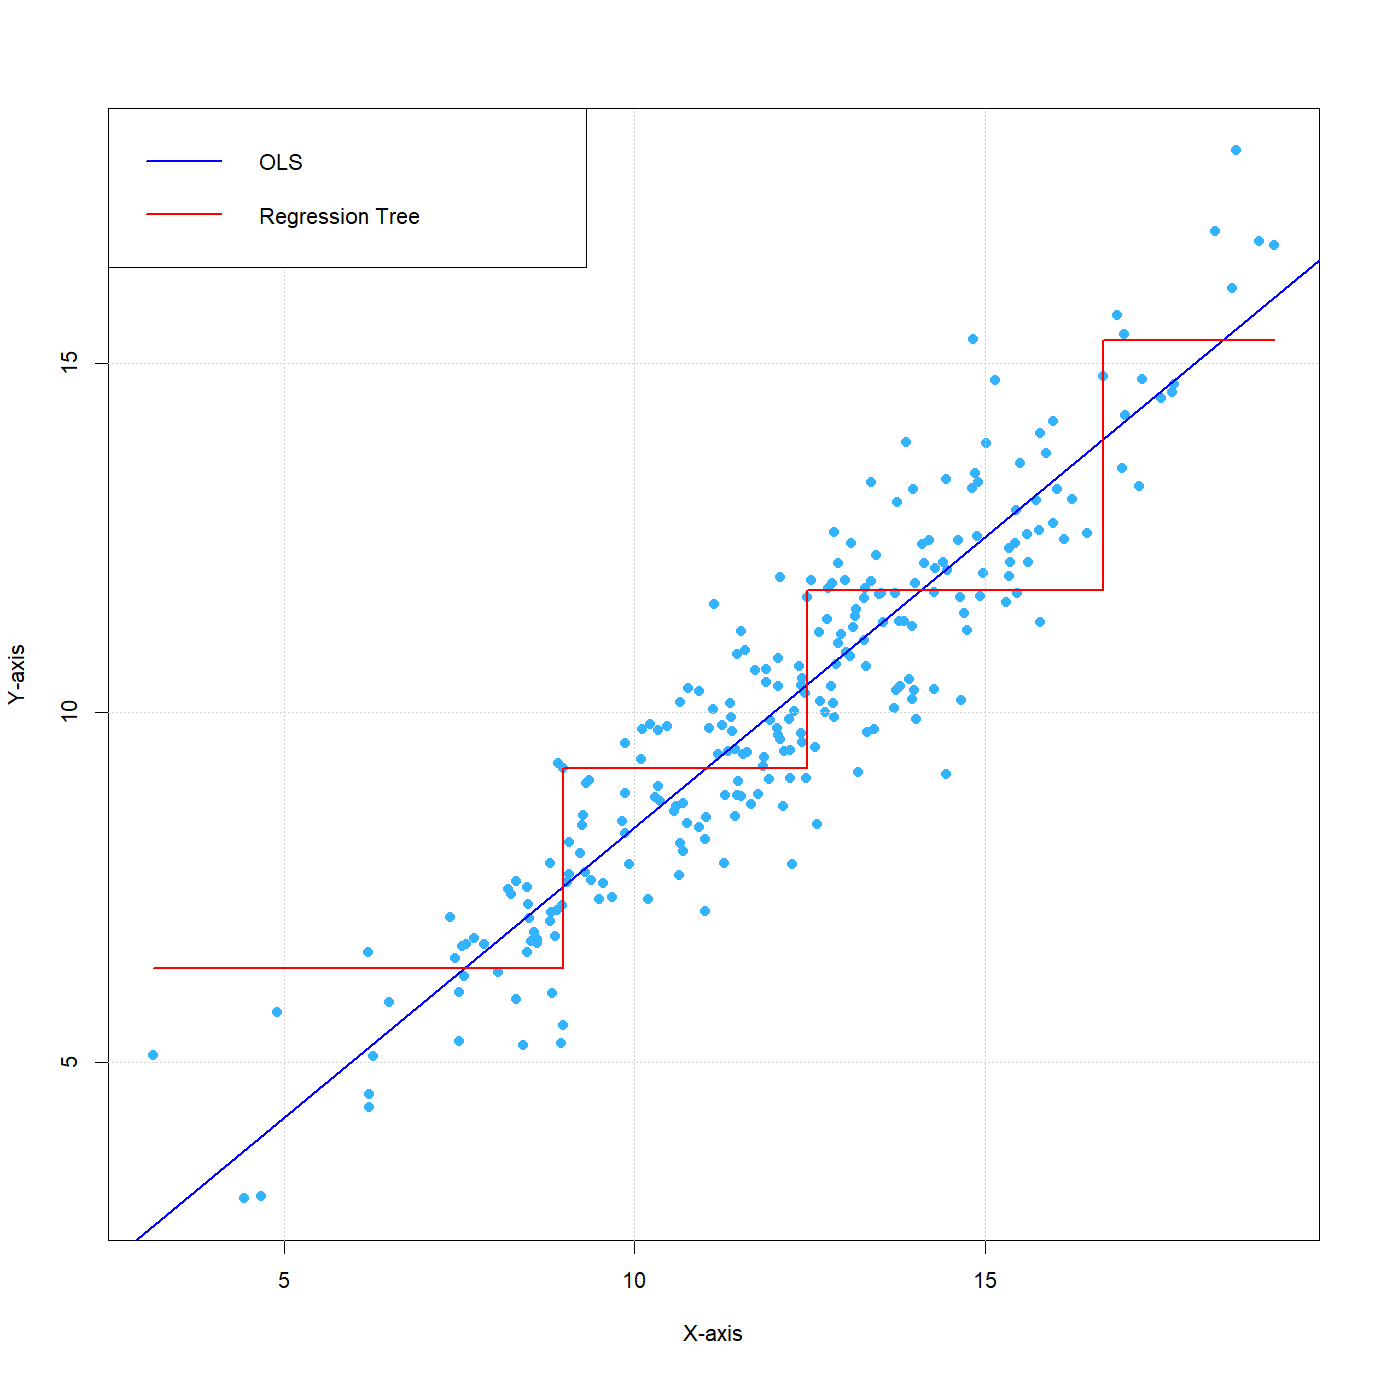
\includegraphics[width=1\linewidth]{OLS vs Tree.png}
            \caption{Linear Relation between Variables}
            \label{fig:sub4}  % Changed label to be unique
            \end{figure}
        \end{column}
        \begin{column}{0.5\textwidth}
        
            \begin{itemize}
                        \vspace{0.7cm}

            \item We will run all simulations 400 times.
                 \item For now the regression trees will have 4 terminal Nodes.
                \item And we will always compare the Mean Squared Error (MSE).
                \vspace{1cm}
                \item \textbf{Results:}
                \item \textbf{MSE} for OLS model: \textbf{0.9917} 
                \item \textbf{MSE} for regression tree model: \textbf{1.4935} 
            \end{itemize}
        \end{column}
    \end{columns}
\end{frame}



\begin{frame}{Simulation: Non-linear Data}
    
        \begin{figure}
            \centering
            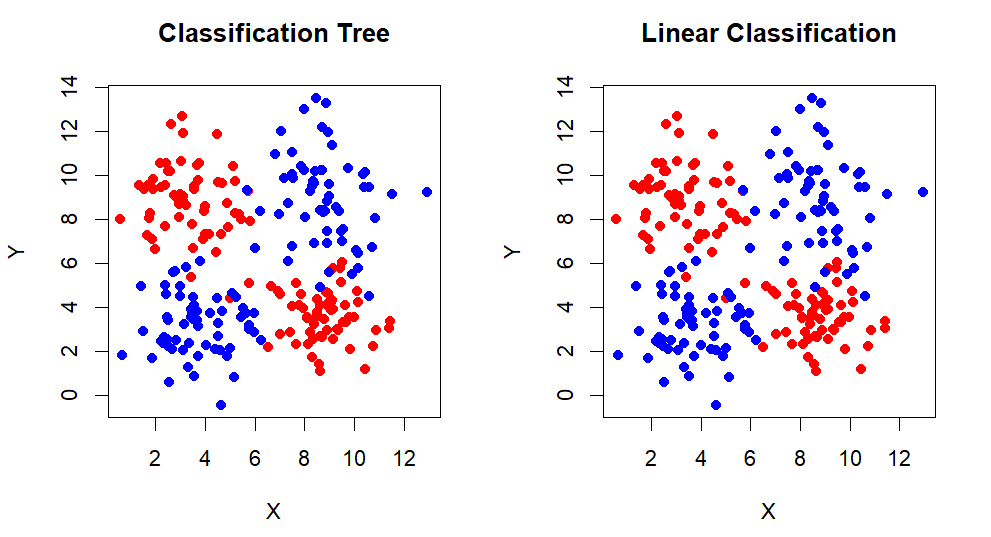
\includegraphics[scale=0.6]{NLD.png}
            \caption{Data with non-linear relationship}
            \label{fig:sub5}  % Changed label to be unique
        \end{figure}
        \vspace{-0.5cm}
        \begin{itemize}
        \item Non-Linear Data generated using 4 normal distributions
        \item NW \& SE = red, NE \& SW = blue
    \end{itemize}
\end{frame}


\begin{frame}{Simulation: Non-linear Data}
    \begin{figure}
        \centering
        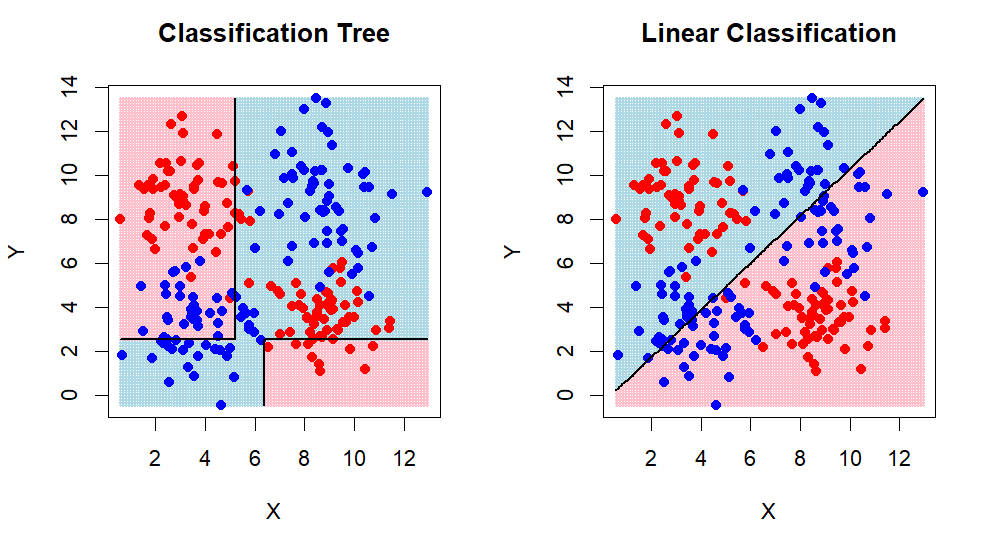
\includegraphics[scale=0.6]{NLD Pred.png}
        \caption{Data with Prediction}
        \label{fig:sub6}  % Changed label to be unique
    \end{figure}
    \vspace{-0.5cm}
    \begin{itemize}
        \item Classification Tree MSE: 0.3757
        \item Linear Classification MSE: 0.5103
        \item \textbf{Trees capture interaction:} e.g. Large Y is only indicative of red if X is small.
    \end{itemize}
\end{frame}






\begin{frame}{Two Problems with Regression Trees}
    \begin{figure}
        \centering
        \begin{subfigure}{.45\textwidth}
            \centering
            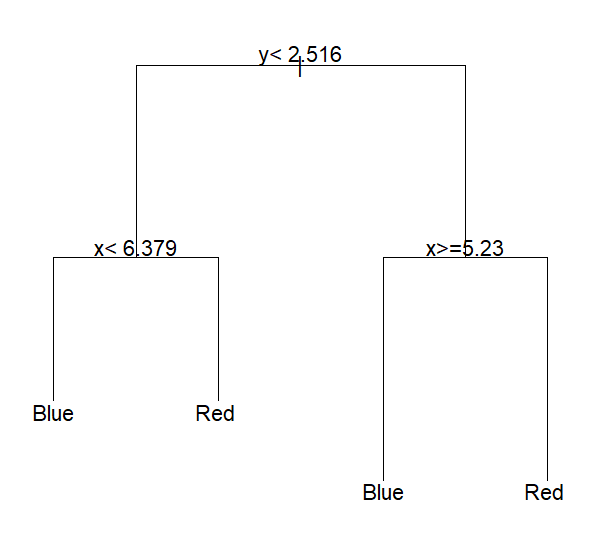
\includegraphics[width=1\linewidth]{Greedy Classification Tree.png}
            \caption{Greedy Classification Tree}
            \label{fig:sub7}  % Changed label to be unique
        \end{subfigure}%
        \begin{subfigure}{.45\textwidth}
            \centering
            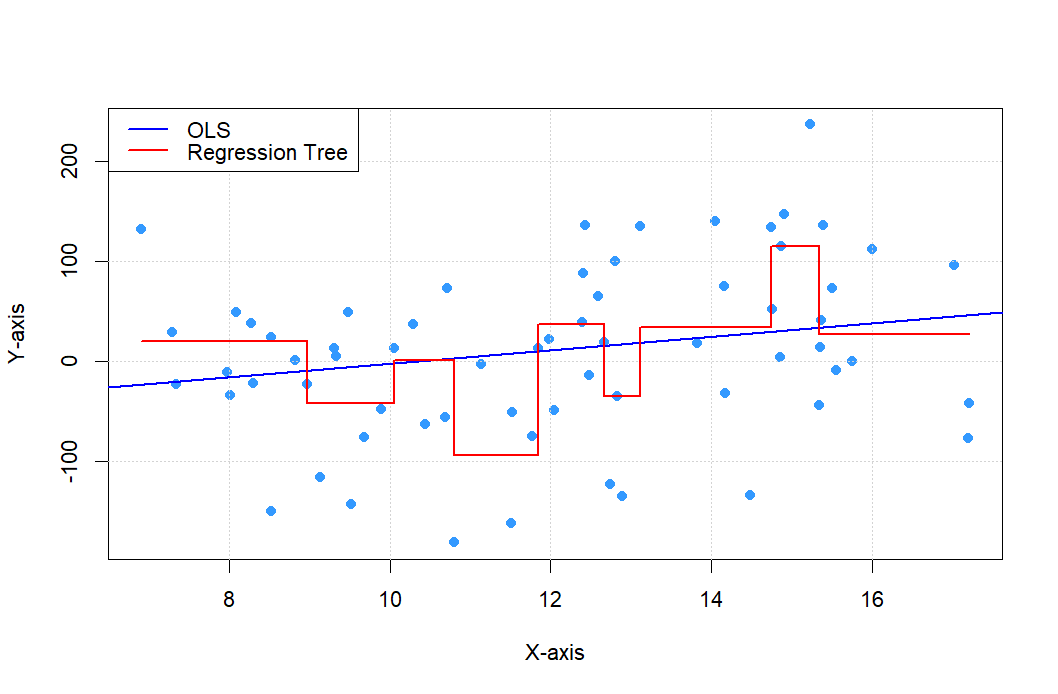
\includegraphics[width=1\linewidth]{Better overfitting.png}
            \caption{Better Overfitting}
            \label{fig:sub8}  % Changed label to be unique
        \end{subfigure}
        \caption{Two Problems that can arise with Trees}
        \label{fig:sub9}  % Changed label to be unique
    \end{figure}
    \begin{itemize}
        \item Overfitting and non-Optimal Splitting
    \end{itemize}
\end{frame}


\begin{frame}{Pruning}
    \begin{itemize}
        \item \textbf{Cost complexity pruning} counteracts overfitting by removing non-essential splits.
        \item Lets us grow a large Tree and then 
        \begin{align*}
            \sum_{m=1}^{|T|} \sum_{i: x_i \in R_m} (y_i - \hat{y}_{R_j})^2 + \alpha|T|.
        \end{align*}
    \begin{itemize}
        \item Select a parameter \( \alpha \).
        \item For each \( \alpha \), find the subtree that minimizes the cost.
           \item Use cross-validation to select the best \( \alpha \).
         \item Instead of evaluating a Model on the data we trained it on we evaluate it on a separate set.
        \end{itemize}
        \item \textbf{Objective:} Achieve a good tradeoff between bias and variance.
       \item Large \( \alpha \) results in very small trees, small \( \alpha \) in larger trees.
    \end{itemize}
\end{frame}


\begin{frame}{Simulation: Finding the optimal Tree size}
    \begin{figure}
        \centering
        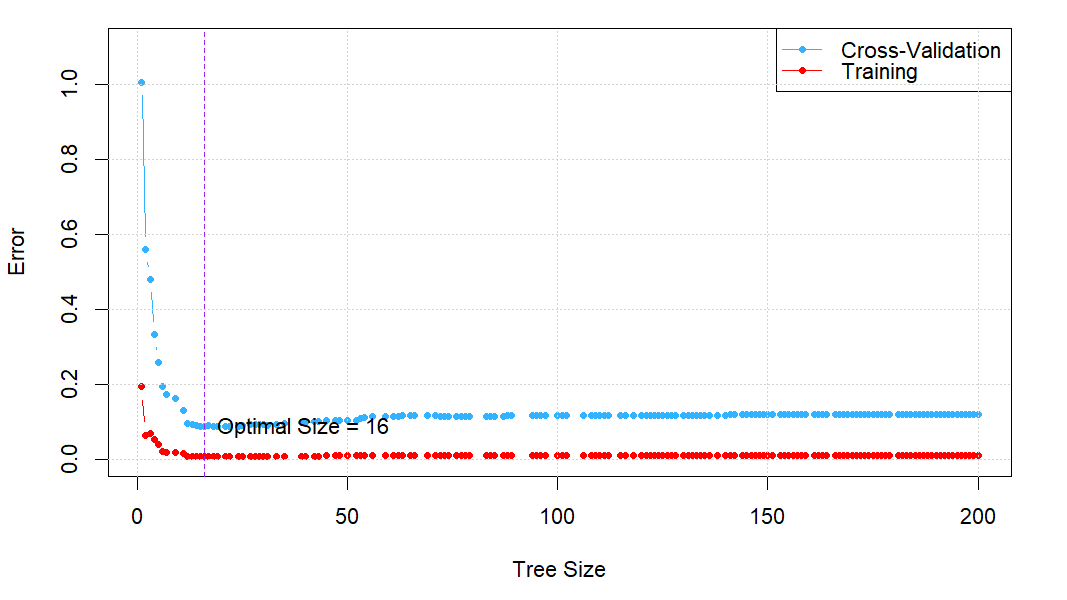
\includegraphics[scale=0.40]{Pruning.png}
        \caption{Training and Cross-Validation Error}
        \label{fig:sub10}  % Changed label to be unique
    \end{figure}
    \begin{itemize}
        \item Pruning helps against overfitting and improves overall performance
        \item Original Tree MSE on Test set = 198.2861 
        \item Pruned Tree MSE on Test set = 173.861 
        \item Sweet spot balances variance and bias, minimizing overfitting.
        \item Training set used to build model, test set to evaluate performance
    \end{itemize}
\end{frame}


\begin{frame}{Ensemble methods}
    \begin{itemize}
        \item Even with pruning trees often perform worse than linear other ML methods
        \item Ensemble methods improve results by combining many regression trees. Each one contributes a small part to the overall prediction.
        \item Each tree can be independent of previous trees (e.g. Random Forests)
        \item Or can be grown on the residuals of the current fit (e.g. Bayesian Additive Regression Trees (BART))
    \end{itemize}
\end{frame}


\begin{frame}{BART}
    \begin{itemize}
        \item BART models the response as a sum of many tree-based models plus noise.
        \item \textbf{Model:}
        \begin{equation}
            Y_i = \sum_{j=1}^{m} g(X_i; T_j, M_j) + \epsilon_i.
        \end{equation}
        \item BART calculates the residuals of the current sum of Trees.
        \item Then modifies one Tree to decrease the residuals.
        \item Then take the average over all but the burn-in iterations.
        \item Unlike single trees, BART avoids overfitting by averaging the predictions of many trees.
        \item BART provides a probabilistic prediction, giving a measure of uncertainty.
    \end{itemize}
\end{frame}


\begin{frame}{Conclusion and Discussion}
    \begin{itemize}
        \item Regression trees are powerful for non-linear and interactive effects.
        \begin{itemize}
            \item Will often outperform linear regression.
        \end{itemize}
        \item They are also very easy to interpret.
        \item Trees require pruning to combat overfitting.
        \item By averaging independent Trees or fitting trees on the residuals ensemble methods can improve results.
        \item BART is a sophisticated method offering good results in many scenarios.
    \end{itemize}
\end{frame}

\begin{frame}{References}
    \begin{itemize}
        \item James, G., Witten, D., Hastie, T., Tibshirani, R. (2021). An Introduction to Statistical Learning with Applications in R (Second Edition). Springer.
        \item Tan, Y. V., Roy, J. (2019). Bayesian additive regression trees and the General BART model. Statistics in Medicine, Band/Volume 38(25), 5048-5069.
        \item Chipman, H. A., George, E. I., McCulloch, R. E. (2010). BART: Bayesian additive regression trees. The Annals of Applied Statistics, Band/Volume 4(1), 266-298.
        \item Townshend, R. Lecture 10 - Decision Trees and Ensemble Methods | Stanford CS229: Machine Learning (Autumn 2018). https://www.youtube.com/watch?v=wr9gUr-eWdA, accessed 21.05.24.
    \vspace{0.5cm}

        \item All images were made using R.
        \item Also thanks to Claude and ChatGPT for making \LaTeX\ a lot nicer to use.
    \end{itemize}
\end{frame}
\end{document}